\documentclass[a4paper]{article}
\usepackage[portuguese]{babel}
\usepackage[utf8]{inputenc}
\usepackage{amsmath}
\usepackage{graphicx}
\usepackage[margin=2cm]{geometry}
\setlength{\parindent}{0cm}
\usepackage{setspace}
\usepackage[colorinlistoftodos]{todonotes}
\usepackage{subfig}
\usepackage{pdfpages}
\usepackage{placeins}
\usepackage{indentfirst}
\usepackage{float}

\begin{document}
\onehalfspace
% Capa
\begin{titlepage}
    \begin{center}
       {\Large UNIVERSIDADE FEDERAL DO PARANÁ}\\[3cm]
       {\Large BRUNA RIBEIRO RESENDE\\[0.5cm]WENDEURICK SILVERIO}\\[8cm]
        {\Large PROJETO DE CONVERSORES CC-CC} \\[0.5cm]
        {\Large CONVERSOR ELEVADOR DE TENSÃO (BOOST)} \\[8cm]
      %  {\Large CONTROLE DE INCLINAÇÃO DE PLATAFORMA \\[0.5cm]COM SENSOR DE ULTRASSOM}\\[6cm]
        {\Large CURITIBA\\[0.5cm]2018}
        \vfill
    \end{center}
\end{titlepage}

\begin{titlepage}
    \begin{center}
       
       {\Large BRUNA RIBEIRO RESENDE\\[0.5cm]WENDEURICK SILVERIO}\\[6cm]
        {\Large PROJETO DE CONVERSORES CC-CC} \\[0.5cm]
        
      {\Large CONVERSOR ELEVADOR DE TENSÃO (BOOST)}\\[1cm]
      \end{center}

  \hspace{.6\textwidth} %posiciona a minipage
   \begin{minipage}{.45\textwidth}
   \large Relatório apresentado à disciplina de Conversores CC-CC e Inversores do curso de Engenharia Elétrica do Departamento de Engenharia Elétrica, Setor de Tecnologia da Universidade Federal do Paraná.\\[0.5cm]
Orientador: Prof. Dr. João Américo Vilela Júnior.\\[6cm]
  \end{minipage}
  \vfill

      \begin{center}
      {\Large CURITIBA\\[0.5cm]2018}
        \vfill
      \end{center}
            
    
\end{titlepage}

{\Large
% inserir o sumario
\tableofcontents
\cleardoublepage

%Textos do trabalho
\Large
\section{Introdução}

Por fim, são apresentadas e discutidas as conclusões e observações de cada etapa do desenvolvimento do projeto proposto.

\section{Objetivos}

\subsection{Objetivo Geral}
\Large
A finalidade do projeto apresentado se resume na implementação de uma das topologias de conversor CC-CC, neste caso, o conversor elevador de tensão (\textit{Boost}). Esta implementação seguirá as seguintes especificações:

\begin{table}[H] \large
\centering
\caption{Especificações do Conversor CC-CC Boost}
\label{tab1}
\begin{tabular}{lc}
\multicolumn{2}{c}{\textbf{Parâmetros de Implementação}}     \\
\hline
Tensão de Entrada       & $9-18V_{cc}$ \\
Tensão de Saída         & $24V_{cc}$   \\
Frequência de Comutação & $250kHz$        \\
Potência do Conversor   & $30W$ \\ \hline
\end{tabular}
\end{table}

\subsection{Objetivos Específicos}

\begin{itemize}
\item Especificação dos componentes do conversor;
\item Projeto do indutor;
\item Definição e simulação do compensador;
\item Layout e confecção da placa de circuito impresso;
%\item Simulação do conversor;
\item Testes em bancada para verificação do funcionamento do conversor \textit{Boost} de acordo com as especificações do projeto.
\end{itemize}

\section{Especificação de Componentes do Conversor}
Nesta seção é realizado o levantamento dos dados necessários para a determinação dos componentes de um conversor CC-CC elevador (\emph{Boost}) (Figura \ref{fig:sch}), cuja a especificação é dada a seguir: $V_{in} = 9-18V$,
$V_{out} = 24V$, $P = 30W$ e $Freq = 250k Hz$.
\FloatBarrier
\begin{figure}[H]
	\centering
	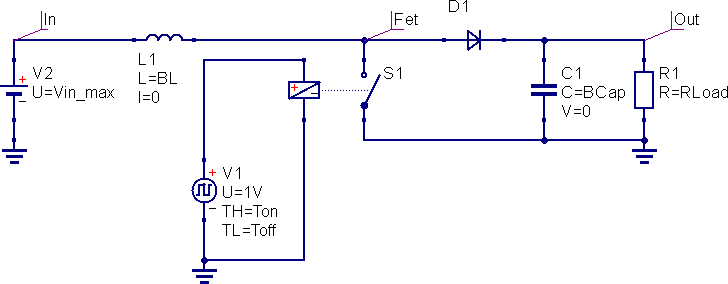
\includegraphics[width=0.85\textwidth]{sch.png}
	\caption{Esquemático do conversor Boost.}
	\label{fig:sch}
\end{figure}
\FloatBarrier
A partir desses parâmetros, tem-se os valores da carga e sua corrente média:

\begin{equation}
\label{eq:r_out}
\begin{split}
R_{out} & = \frac{V_{out}^{2}}{P} \\
& = \frac{{24}^{2}}{30} = 19,2 \Omega
\end{split}
\end{equation}

\begin{equation}
\label{eq:i_out_med}
\begin{split}
I_{{out}_{med}} & = \frac{P}{V_{out}} \\
& = \frac{30}{24} = 1,250 A
\end{split}
\end{equation}

Com isso, através do \textit{software} Qucs, simulou-se o circuito da Figura \ref{fig:sch}, obtendo-se os parâmetros a seguir.

%\pagebreak

\begin{enumerate}
% ---------------------------------------------
\item Capacitor
\begin{enumerate}
\item Capacitância \\
A escolha da capacitância leva em conta a variação da tensão de saída (${\triangle}_{V_{out}}$) e a razão cíclica (\emph{D}) da chave. \\
O ciclo de trabalho foi calculado para o pior caso, ou seja, quando \emph{D} assume seu valor máximo (quando a tensão de entrada assume o valor mínimo):

\begin{equation}
\label{eq:d_max_cap}
\begin{split}
D & = 1-\frac{V_{in}}{V_{out}} \\
& = 1-\frac{9}{24} = 62.5\%
\end{split}
\end{equation}

Para este projeto, adotou-se a variação de tensão igual a 4\%. A Equação \ref{eq:cap} apresenta o cálculo do valor mínimo da capacitância.

\begin{equation}
\label{eq:cap}
\begin{split}
C_{ap} & \geq \frac{D_{max} \cdot I_{out}}{{\triangle}_{V_{out}} \cdot f_{req}} \\
& = \frac{62,5\% \cdot 1,250}{4\% \cdot 250k} = 78,125\mu F
\end{split}
\end{equation}

\item Tensão máxima \\
Através da simulação, obteve-se a tensão máxima que o capacitor deve suportar (37,5V, quando $V_{in} = 18V$).
\FloatBarrier
\begin{figure}[H]
	\centering
	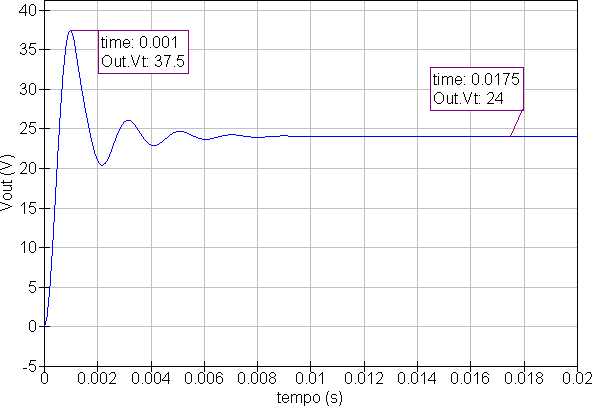
\includegraphics[width=0.8\textwidth]{vout_vinmax.png}
	\caption{Pico de tensão sobre a carga/capacitor.}
	\label{fig:vout_vinmax}
\end{figure}
\FloatBarrier
\item ESR máxima \\
Neste projeto, adotou-se 4\% como sendo o valor da máxima variação da corrente de saída (${\triangle}_{I_{out}}$). A Equação \ref{eq:esr_cap} apresenta o cálculo da resistência séria máxima do capacitor.

\begin{equation}
\label{eq:esr_cap}
\begin{split}
ESR & \leq \frac{{\triangle}_{V_{out}}}{{\triangle}_{I_{out}}} \\
& = \frac{4\%}{4\%} = 1 \Omega
\end{split}
\end{equation}

\end{enumerate}
% ---------------------------------------------
\item Indutor
\begin{enumerate}
\item Indutância \\
O cálculo para o valor mínimo da indutância (Equação \ref{eq:ind}) foi feito sobre o ponto onde o produto ($D \cdot V_{in}$) atinge seu valor máximo:

\begin{equation}
\label{eq:max_d_vin}
\begin{split}
max\left\{ D \cdot V_{in} \right\} & = max\left\{ \frac{(V_{out}-V_{in})}{V_{out} } \cdot V_{in} \right\} \\
& = max\left\{ \frac{(24-V_{in})}{24} \cdot V_{in} \right\} = 6 \rightarrow V_{in} = 12 \rightarrow D = 50\%
\end{split}
\end{equation}

\begin{equation}
\label{eq:ind}
\begin{split}
L & \geq \frac{D \cdot V_{in}}{{\triangle}_{I_{L}}\cdot f_{req}} \\
& = \frac{6}{{4\%}\cdot 250k} = 600 \mu H
\end{split}
\end{equation}

%\pagebreak

\item Corrente média \\
\label{subsub:corrente-media}
Através da simulação, obteve-se a corrente média que o indutor deve suportar (4,51A, quando $V_{in} = 9V$).

\begin{figure}[H]
	\centering
	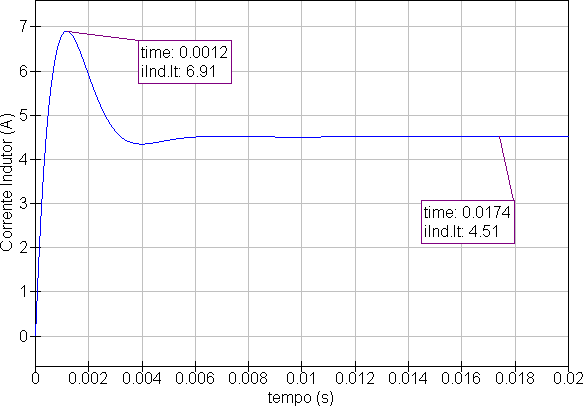
\includegraphics[width=0.67\textwidth]{iind_vinmin.png}
	\caption{Corrente média sobre o indutor.}
	\label{fig:iind_med}
\end{figure}
\pagebreak
\item Corrente máxima \\
\label{subsub:corrente-max}
Através da simulação, obteve-se a corrente máxima que o indutor deve suportar (8,22A, quando $V_{in} = 18V$).
\FloatBarrier
\begin{figure}[H]
	\centering
	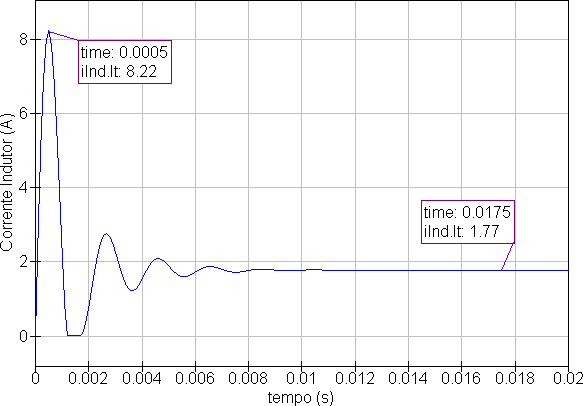
\includegraphics[width=0.67\textwidth]{iind_vinmax.png}
	\caption{Corrente máxima sobre o indutor.}
	\label{fig:iind_max}
\end{figure}
\FloatBarrier
\end{enumerate}
% ---------------------------------------------
\item Diodo
\begin{enumerate}
\item Corrente média e corrente máxima\\
A corrente no diodo é aproximadamente igual à corrente sobre a carga (desconsiderando os picos de carga sobre o capacitor). 
\FloatBarrier
\begin{figure}[H]
	\centering
	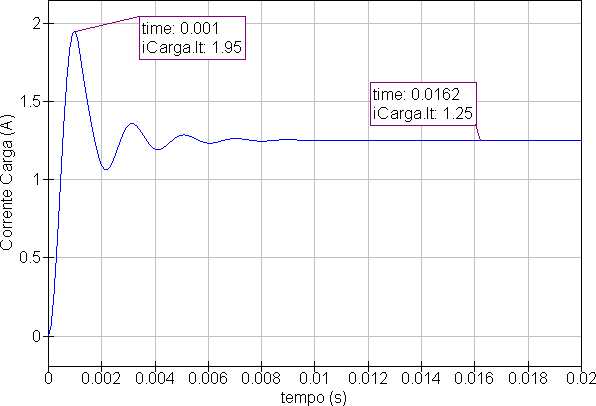
\includegraphics[width=0.7\textwidth]{icarga_vinmax.png}
	\caption{Corrente sobre o diodo/carga.}
	\label{fig:idiodo}
\end{figure}
\FloatBarrier
Através da simulação, obteve-se a corrente média e máxima que o diodo deve suportar (1,25A e 1,95, respectivamente, quando $V_{in} = 18V$).

\item Tensão reversa máxima \\
Através da simulação, obteve-se a máxima tensão reversa que o diodo deve suportar (35,6V, quando $V_{in} = 18V$).
\FloatBarrier
\begin{figure}[H]
	\centering
	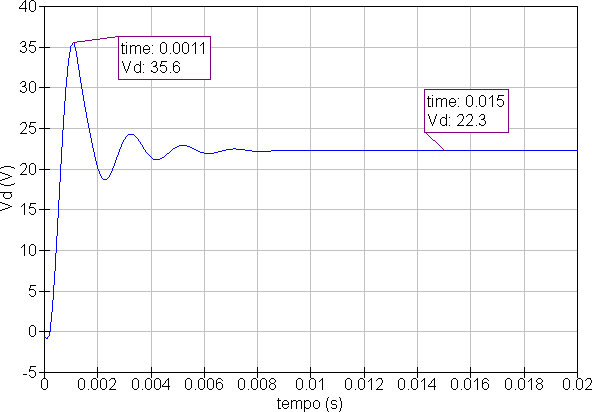
\includegraphics[width=0.62\textwidth]{vdrev_vinmax.png}
	\caption{Tensão reversa sobre o diodo.}
	\label{fig:vdrev}
\end{figure}
\FloatBarrier
\end{enumerate}
% ---------------------------------------------
\item Mosfet
\begin{enumerate}
\item Corrente média \\
Através da simulação, obteve-se a corrente média que a chave deve suportar (4,54A, quando $V_{in} = 9V$).
\FloatBarrier
\begin{figure}[H]
	\centering
	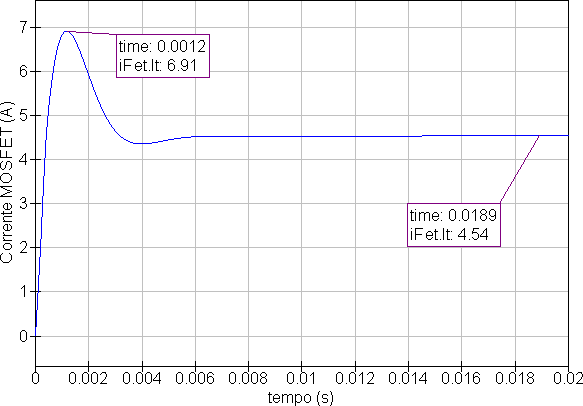
\includegraphics[width=0.62\textwidth]{ifet_vinmin.png}
	\caption{Corrente média sobre a chave.}
	\label{fig:ifet_med}
\end{figure}
\FloatBarrier
\pagebreak
\item Corrente máxima \\
Através da simulação, obteve-se a corrente máxima que a chave deve suportar (8,22A, quando $V_{in} = 18V$).
\FloatBarrier
\begin{figure}[H]
	\centering
	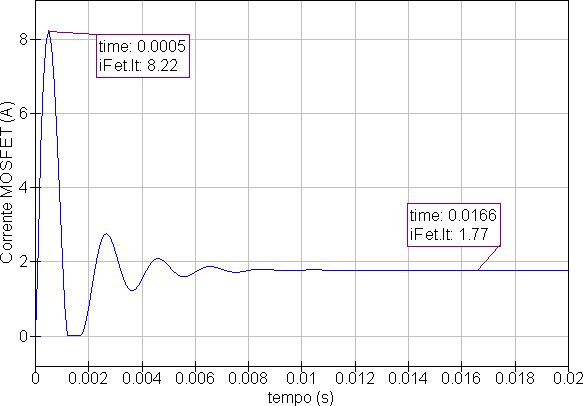
\includegraphics[width=0.67\textwidth]{ifet_vinmax.png}
	\caption{Corrente máxima sobre a chave.}
	\label{fig:ifet_max}
\end{figure}
\FloatBarrier
\item Tensão Dreno-Fonte
\label{subitem:vds}

Através da simulação, obteve-se a tensão máxima que a chave deve suportar (8,22V, quando $V_{in} = 18V$).

\begin{figure}[H]
	\centering
	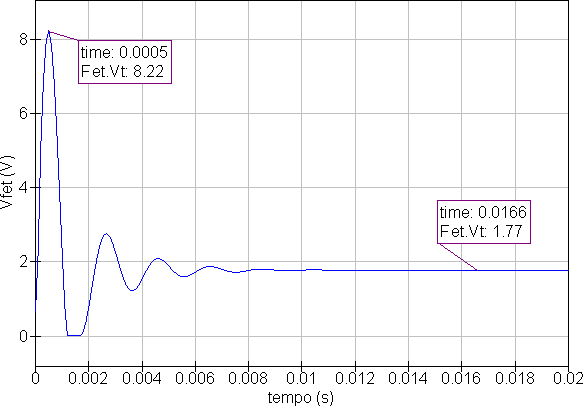
\includegraphics[width=0.67\textwidth]{vfet_vinmax.png}
	\caption{Tensão máxima sobre a chave.}
	\label{fig:vfet_max}
\end{figure}

\end{enumerate}

\end{enumerate}

\subsection*{Escolha dos componentes}
A partir dos dados obtidos através dos cálculos, da simulação e da disponibilidade, foram definidos os seguintes componentes:

\begin{enumerate}

\item Capacitor
\begin{itemize}
\item Fabricante: Nichicon
\item Part number: UVR1H470MED1TD
\item Capacitância: 2x$47 \mu F$ $\pm 20\%$ (2 em paralelo)
\item Tensão máxima de operação: 50V
\item ESR: não especificada pelo fabricante. Medida: $490 m\Omega$.
\end{itemize}

\item Diodo
\begin{itemize}
\item Fabricante: Vishay General Semiconductor
\item Part number: SB260
\item Queda de tensão: 680mV @ 2A
\item Corrente média: 2,0A
\item Pico máximo de corrente: 60A @ 8,3ms
\item Máxima tensão reversa: 60V
\end{itemize}

\item Mosfet
\begin{itemize}
\item Fabricante: Infineon Technologies	
\item Part number: IRFZ44EPBF
\item Corrente média: 48A
\item Pico máximo de corrente: 192A
\item Tensão máxima entre dreno e fonte: 60V
\item Resistência Dreno-Fonte modo triodo: $23m\Omega$ @$V_{GS} = 10V, I_D = 29A$
\item Tensão de limiar no \emph{gate}: 2V - 4V
\end{itemize}

\end{enumerate}

\clearpage

\section{Projeto do Indutor}

Para o cálculo do número de espiras do indutor em questão, foi utilizada a metodologia a partir do comprimento de entreferro. Assim, o carretel foi projetado de forma que o comprimento do entreferro fosse igual a 1,6mm, ou seja:

\begin{equation*}
\frac{l_g}{2} = 0,8mm
\end{equation*}

\begin{equation*}
N = \sqrt{\frac{l_g \cdot L}{\mu_0 \cdot A_e}} = \sqrt{\frac{1,6 \cdot 10^{-3} \cdot 600 \cdot 10^{-6}}{4 \cdot \pi \cdot 10^{-7} \cdot 1,7 \cdot 10^{-4}}} = 67,09\text{ espiras}
\end{equation*}

Onde:
\begin{itemize}
\item L - indutância [H]
\item $\mu_0$ - permeabilidade magnética do vácuo [H/m]
\item $A_e$ - área do núcleo [$m^2$]
\end{itemize}

Assim, utilizou-se 68 espiras para a construção do indutor. No entanto, é necessário verificar se a densidade de fluxo $B_{max}$ não ultrapassa o valor de 0,3T, provocando a saturação do núcleo. Como pode ser observado na Equação \ref{eq:b-max-erro}, não haverá saturação.

\begin{equation}
\label{eq:b-max-erro}
B_{max} =  \frac{L \cdot I_{pico}}{N \cdot A_e} = \frac{600 \cdot 10^{-6} \cdot 1,275}{68 \cdot 1,7 \cdot 10^{-4}} = 0,066T
\end{equation}

Foi então analisada a área disponível para o número de espiras calculado, pela equação abaixo, considerando a densidade de corrente máxima $J_{max}$ igual a $450 A/cm^2$ e a corrente eficaz $I_{ef}$ igual a 1,25 A.

\begin{equation}
\label{eq:area-erro}
A_{t} = \frac{I_{ef}}{J_{max}} = 0,0027 cm^2 = 0,27 mm^2
\end{equation}

No entanto, a corrente utilizada foi equivocada, uma vez que se considerou a corrente de saída média e não a corrente máxima que efetivamente passa pelo indutor em regime permanente. O erro foi identificado após a implementação do conversor e durante os ensaios, onde o indutor aqueceu. Refazendo os cálculos para verificar a dimensão do erro, utilizou-se a corrente máxima, na condição da tensão de entrada mínima, igual a 3,33 A:

\begin{equation}
\label{eq:area-erro}
A_{t} = \frac{I_{max}}{J_{max}} = 0,0074 cm^2 = 0,74 mm^2
\end{equation}

Dessa forma, seria necessária a utilização de um condutor $AWG_{18}$, cuja seção é de $0,82mm^2$.

Porém, como se está operando em frequência elevada para eletrônica de potência, deve-se considerar o efeito pelicular, utilizando a frequência do projeto igual a 250kHz.

\begin{equation*}
\triangle= \frac{7,5}{\sqrt{f}} = 0,015 cm = 0,15mm
\end{equation*}

Como o raio do condutor deve ser menor que $\triangle$, o condutor mais indicado seria o $AWG_{29}$, cujo raio é de 0,14295mm. No entanto, havia a disponibilidade do condutor $AWG_{30}$ e assim, seria necessária a utilização de um número de condutores em paralelo obtido pela equação:

\begin{equation*}
n_{cp} = \frac{AWG_{18}}{AWG_{30}} = 16,07 \approx 17 \text{ condutores em paralelo}
\end{equation*}

Assim, realizando os mesmos cálculos, porém com o valor da corrente média de saída, foi obtido um número de 3 condutores em paralelo utilizando o $AWG_{30}$, valor muito distante do necessário. Assim, o indutor foi construído com o condutor $AWG_{30}$ e 3 condutores em paralelo.

Após a construção do indutor, a medição de sua indutância indicou aproximadamente $643,7\mu H$. Além disso, a ESR medida foi igual a $480m\Omega$. (obs.: a Seção \ref{sec:conclusoes} aborda novamente o projeto do indutor).

\clearpage

\section{Projeto do Compensador}

\subsection{Circuito de Controle}

O compensador escolhido foi o do Tipo 3, cujo circuito e função transferência são apresentados nas Figuras \ref{fig:sch-comp} e \ref{fig:tf-comp}, respectivamente.

\begin{figure}[H]
	\centering
	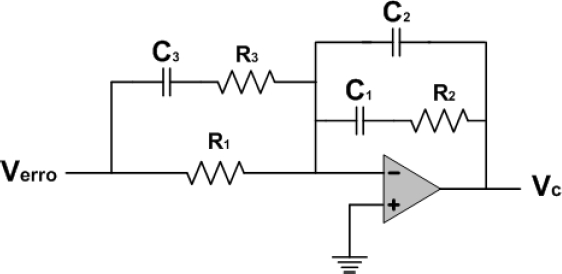
\includegraphics[width=0.4\textwidth]{sch-comp.jpg}
	\caption{Circuito do Compensador Tipo 3.}
	\label{fig:sch-comp}
\end{figure}

\begin{figure}[H]
	\centering
	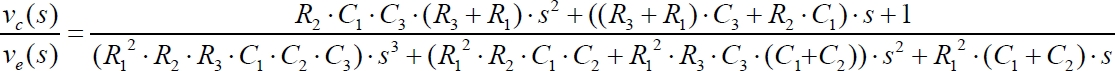
\includegraphics[width=0.98\textwidth]{tf-comp.jpg}
	\caption{Função transferência do Compensador Tipo 3.}
	\label{fig:tf-comp}
\end{figure}

A equação \ref{eq:tfboost} apresenta a função transferência do conversor \emph{Boost}.

\begin{equation}
\label{eq:tfboost}
\begin{split}
G_{Boost} ={\frac{V_{in}}{L \cdot C \cdot \left(1-D\right)^{2}}} \cdot \frac{ \left( - \frac{R_{SE} \cdot L \cdot C \cdot s^2}{R_0} + \left( R_{SE} \cdot C - \frac{L}{R_0} \right) \cdot s+1 \right) }{\left( s^2 + \left( \frac{1}{R_0 \cdot C} + \frac{R_{SE}}{L} \right) \cdot s + \frac{1}{L \cdot C} \right)}
\end{split}
\end{equation}

Onde
\begin{itemize}
\item \textbf{V\textsubscript{in}}: tensão de entrada
\item \textbf{L}: valor do Indutor \emph{Boost}
\item \textbf{C}: valor do Capacitor \emph{Boost}
\item \textbf{R\textsubscript{SE}}: ESR do capacitor
\item \textbf{R\textsubscript{0}}: carga do circuito
\item \textbf{D}: razão cíclica
\item \textbf{s}: variável no plano complexo (frequência complexa)
\end{itemize}

O projeto do compensador foi dado no ponto $Vin = 13,5V$. Assumindo esse valor na Equação \ref{eq:d_max_cap}, tem-se o valor da razão cíclica igual a $D = 0,4375$.

A fim de se obter valores mais próximos para o caso real, os componentes físicos foram medidos e o compensador foi projetado levando em conta esses valores.

\begin{itemize}
\item L = $643,7\mu H$
\item C = $2 \cdot 47\mu = 94\mu F$ (capacitores em paralelo)
\item R\textsubscript{SE} = $0,49 \Omega / 2 = 0,245 \Omega$ (capacitores em paralelo)
\item R\textsubscript{0} = $19,2 \Omega$
\end{itemize}

Com isso, obteve-se os diagramas de Bode em malha aberta, apresentados na Figura \ref{fig:bode}. Logo após, escolheu-se 2,08kHz para ser a frequência de corte em malha fechada, ponto onde a fase é de 166º (-194º) e magnitude é de 14dB (5,01V/V).

\begin{figure}[H]
	\centering
	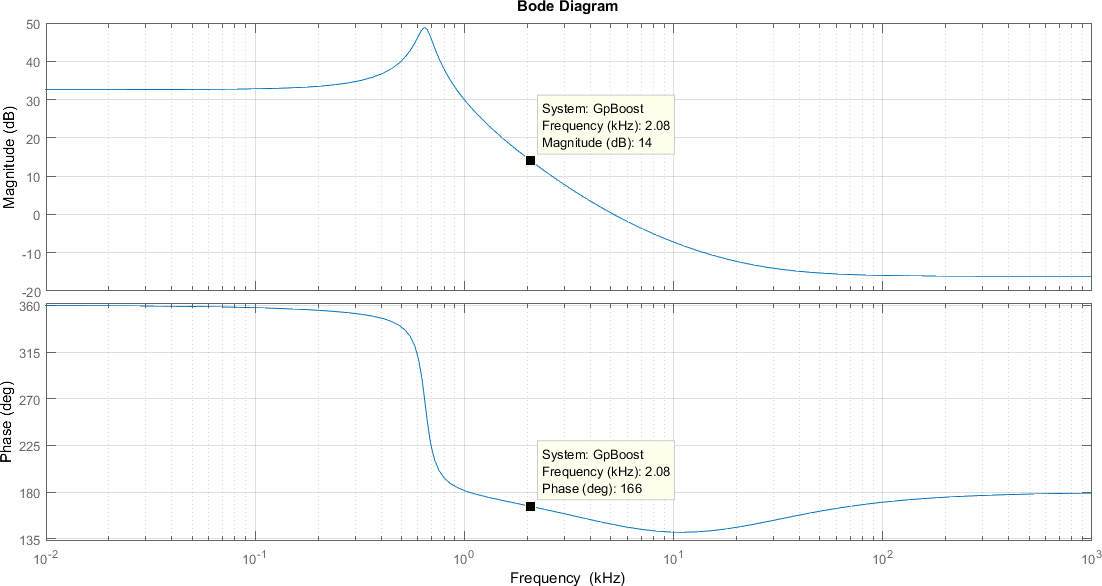
\includegraphics[width=0.98\textwidth]{GpBoost_freq_corte_escolhida.png}
	\caption{Diagramas de Bode da função transferência do conversor \emph{Boost}.}
	\label{fig:bode}
\end{figure}

Optou-se pela margem de fase igual a 60º. Com isso, obteve-se o avanço de fase, conforme a Equação \ref{eq:avanco-fase}.

\begin{equation}
\label{eq:avanco-fase}
\begin{split}
\phi_{\text{avanço}} & = -90^{\circ} + MF_{desejada} - \angle G_{Boost}\mid_{f_c} \\
& = -90^{\circ} + 60^{\circ} - (-194^{\circ}) = 164^{\circ}
\end{split}
\end{equation}

O ganho do compensador deve ser tal que leve a um ganho unitário em malha fechada, na frequência de corte (Equação \ref{eq:ganho-unit}).

\begin{equation}
\label{eq:ganho-unit}
\begin{split}
\mid G_{FTMA}\left(s\right)\mid_{f_c} = \mid G_{C}\left(s\right)\mid_{f_c} \cdot \mid G_{PWM}\left(s\right)\mid_{f_c} \cdot \mid G_{Boost}\left(s\right)\mid_{f_c} \cdot k = 1
\end{split}
\end{equation}

Substituindo os seguintes valores na Equação \ref{eq:ganho-unit}, obteve-se o \text{Ganho do Compensador} $\mid G_c\left( s \right) \mid_{f_c} = 1,7957V/V$.

\begin{itemize}

\item \text{Ganho da planta do conversor}: $ \mid G_{Boost} \left( s \right) \mid_{f_c} = 5,01$

\item \text{Ganho da modulação PWM}: $\mid G_{PWM}\left( s \right) \mid_{f_c} = 1/V_{triang} = 1/1,8 = 0,5556$

\item \text{Ganho do divisor resistivo de \emph{feedback}}: $ k = 5V / 24V = 0,2 $

\end{itemize}

O fator $k_{pz}$ é dado pela Equação \ref{eq:kpz}.

\begin{equation}
\label{eq:kpz}
\begin{split}
k_{pz} & = \left( \tan \left( \frac{\phi_{\text{avanço}}}{4}+\frac{\pi}{4} \right)  \right)^2 \\
& = \left( \tan \left( \frac{164}{4}+\frac{\pi}{4} \right)  \right)^2 = 204,5091
\end{split}
\end{equation}

Tomando o resistor $R_1 = 510k\Omega$, calculou-se os demais componentes do compensador.

\begin{equation}
\label{eq:comp-c2}
\begin{split}
C_{2} & = \frac{1}{2 \cdot \pi \cdot f_{c} \cdot R_{1} \cdot \mid G_{c} \left( s \right)\mid} \\
& = \frac{1}{2 \cdot \pi \cdot 2,08kHz \cdot 510k\Omega \cdot 1,7957} = 83,550pF
\end{split}
\end{equation}

\begin{equation}
\label{eq:comp-c1}
\begin{split}
C_{1} & = C_{2} \cdot \left( k_{pz}-1 \right) \\
& =  83,550pF \cdot \left( 204,5091 - 1 \right) = 17nF
\end{split}
\end{equation}

\begin{equation}
\label{eq:comp-r2}
\begin{split}
R_{2} & = \frac{\sqrt{k_{pz}}}{2 \cdot \pi \cdot f_{c} \cdot C_{1}} \\
& = \frac{\sqrt{204,5091}}{2 \cdot \pi \cdot 2,08k\Omega \cdot 17nF} = 64,355k\Omega
\end{split}
\end{equation}

\begin{equation}
\label{eq:comp-r3}
\begin{split}
R_{3} & = \frac{R_{1}}{k{pz}-1} \\
& = \frac{510k\Omega}{204,5091-1} = 2,51k\Omega
\end{split}
\end{equation}

\begin{equation}
\label{eq:comp-c3}
\begin{split}
C_{3} & = \frac{1}{2 \cdot \pi \cdot f_{c} \cdot R_{3} \cdot \sqrt{k_{pz}}} \\
& = \frac{1}{2 \cdot \pi \cdot 2,08kHz \cdot 2,51k\Omega \cdot \sqrt{204,5091}} = 2,14nF
\end{split}
\end{equation}

Após os cálculos, foi feita uma aproximação com valores comerciais e/ou disponíveis, através de arranjos série/paralelo, obtendo aos seguintes valores:

\begin{table}[H]
\centering
\caption{aproximação com valores comerciais/disponíveis}
\label{tab:comp-com}
\begin{tabular}{ll}
$R_1 \left( k\Omega \right)$ & 510 \\
$R_2 \left( k\Omega \right)$ & 56 \\
$R_3 \left( k\Omega \right)$ & 2,2 \\
$C_1 \left( nF \right)$ & 17,2 \\
$C_2 \left( pF \right)$ & 94 \\
$C_3 \left( nF \right)$ & 2,2
\end{tabular}
\end{table}

Substituindo as devidas funções transferências no sistema da Figura \ref{fig:sistema-controle}, obteve-se os diagramas de Bode da Figura \ref{fig:bode-controle}.

\begin{figure}[H]
	\centering
	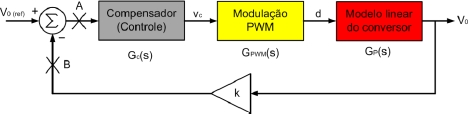
\includegraphics[width=0.9\textwidth]{sistema-controle.jpg}
	\caption{Sistema de controle do conversor \emph{Boost}.}
	\label{fig:sistema-controle}
\end{figure}

\begin{figure}[H]
	\centering
	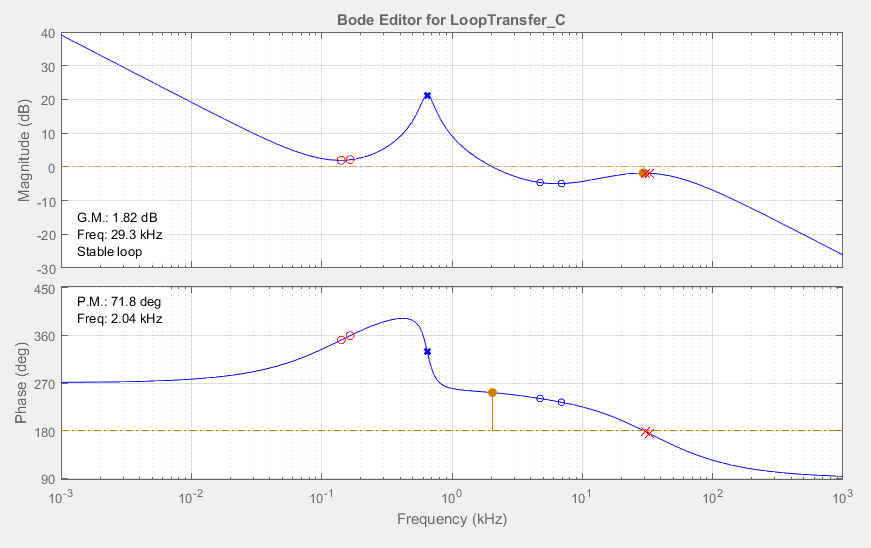
\includegraphics[width=0.99\textwidth]{CompensadorBode.png}
	\caption{Diagramas de Bode do conversor \emph{Boost}.}
	\label{fig:bode-controle}
\end{figure}

\subsection{Frequência de Oscilação}

A implementação do compensador foi realizada através do circuito integrado TL494, cujo diagrama simplificado é apresentado na Figura \ref{fig:tl494}.

\begin{figure}[H]
	\centering
	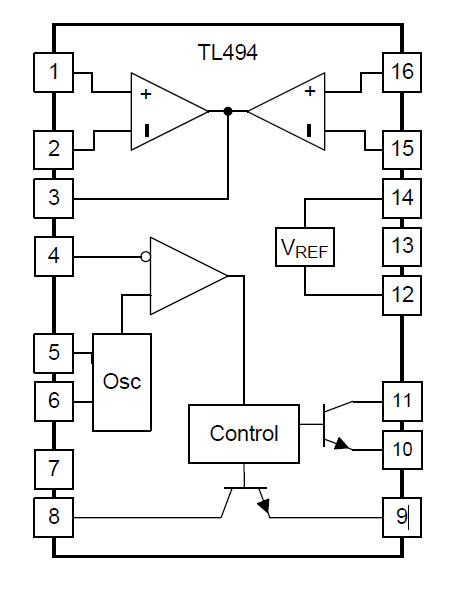
\includegraphics[width=0.35\textwidth]{diag-simp.PNG}
	\caption{Diagrama simplificado do CI TL494.}
	\label{fig:tl494}
\end{figure}

Segundo sua documentação (\emph{datasheet}), a frequência de oscilação é dada pelo inverso do produto de um capacitor ($C_T$) e um resistor ($R_T$), conectados aos pinos 5 e 6, respectivamente. O cálculo para $f_{OSC} \approx 250kHz$ é apresentado na Equação \ref{eq:fosc}.
\begin{equation}
\label{eq:fosc}
\begin{split}
f_{OSC} & = \frac{1}{C_T \cdot R_T} \\
& = \frac{1}{1,8nF \cdot 2,2k\Omega} = 253kHz
\end{split}
\end{equation}

\subsection{Tensão de \emph{feedback}}

A entrada não-inversora do comparador (pino 1) recebe a tensão de \emph{feedback} do conversor \emph{Boost}, devendo ser ajustada à faixa 0V - 5V. Para isso, implementou-se um divisor resistivo, apresentado na Equação \ref{eq:div-res}.

\begin{equation}
\label{eq:div-res}
\begin{split}
V_{feedback_{max}} & = \frac{24V \cdot 1k\Omega}{1k\Omega + 3,8k\Omega}  = 5V
\end{split}
\end{equation}

\subsection{\emph{Soft-start} e tempo-morto}

As técnicas de \emph{soft-start} e tempo-morto são necessárias para mitigar o estresse sobre o \emph{Mosfet} durante a inicialização do sistema, fazendo com que o capacitor \emph{Boost} se carregue lentamente. A Figura \ref{fig:soft-start} apresenta a limitação do ciclo de trabalho em função da tensão aplicada no pino 4 do circuito integrado.

\begin{figure}[H]
	\centering
	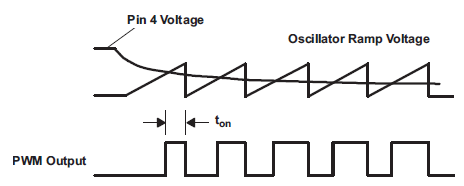
\includegraphics[width=0.65\textwidth]{soft-start.PNG}
	\caption{Controle do ciclo de trabalho.}
	\label{fig:soft-start}
\end{figure}

A entrada do comparador do tempo-morto (pino 4) trabalha com tensões entre 0V e 3,3V, fazendo com que o \emph{Mosfet} seja cortado, proporcionalmente, de 3\% a 100\%, ou seja, a razão cíclica varia entre 0,97 e 0.

A Equação \ref{eq:deadv} apresenta o cálculo para a máxima tensão no pino 4 em função do máximo valor da razão cíclica (escolhido $D = 85\%$).

\begin{equation}
\label{eq:deadv}
\begin{split}
V_{4_{max}} & = \frac{3,3V \cdot \left(0,97-0,85\right)}{0,97} = 0,408V
\end{split}
\end{equation}

Como pode ser notado na Figura \ref{fig:soft-div}, a tensão interna de referência é de 5V, sendo necessário um divisor resistivo para limitar o pino 4 em 0,408V. Assumindo o resistor \emph{shunt} igual a $10k\Omega$, tem-se o seguinte valor do resistor $R_{T_{ss}}$ (Equação \ref{eq:soft-div-res}).

\begin{figure}[H]
	\centering
	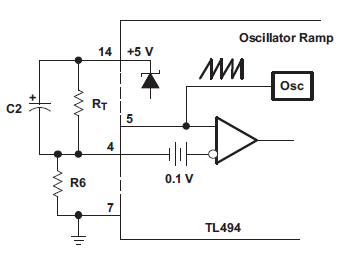
\includegraphics[width=0.5\textwidth]{soft-div.png}
	\caption{Circuito de \emph{soft-start}.}
	\label{fig:soft-div}
\end{figure}

\begin{equation}
\label{eq:soft-div-res}
\begin{split}
R_{T_{ss}} & = R_{shunt} \cdot \left( \frac{V_{ref}}{V_{4_{max}}} - 1\right) \\
& = 10k\Omega \cdot \left( \frac{5V}{0,408V} - 1\right) \approx 110k\Omega
\end{split}
\end{equation}

Para o tempo de \emph{soft-start}, definiu-se o equivalente para 93 ciclos de \emph{clock}, assim, o valor da capacitância é dada pela Equação \ref{eq:soft-cap}.

\begin{equation}
\label{eq:soft-cap}
\begin{split}
C_{ss} & =  \frac{1}{f_{OSC}} \cdot \frac{N_{ciclos}}{R_{T_{ss}}}\\
& = \frac{1}{250kHz} \cdot \frac{93}{110k\Omega} \approx 3,3nF
\end{split}
\end{equation}

A Figura \ref{fig:sch-controle} apresenta o circuito de controle/compensação completo.

\begin{figure}[H]
	\centering
	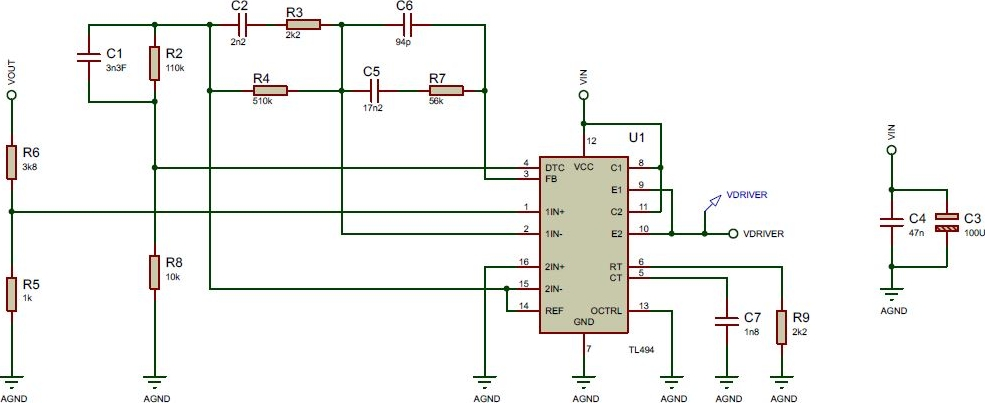
\includegraphics[width=1.0\textwidth]{sch-controle.jpg}
	\caption{Circuito de controle/compensação.}
	\label{fig:sch-controle}
\end{figure}


\clearpage

\section{Placa de Circuito Impresso}

A placa de circuito impresso foi projetada com base em boas práticas de leiaute e alguns cuidados foram tomados em relação à disposição dos circuitos.
\\
\\
O circuito de potência (Figura \ref{fig:sch-pot}) foi projetado com trilhas largas e buscou-se fazê-lo com o menor \emph{loop} possível. Ademais, para diminuir os efeitos da ESR, o capacitor Boost de $78,125\mu F$ foi substituído por 2 capacitores (CB1 e CB2) de $47\mu F$ em paralelo, totalizando $\approx100\mu F$ e metade da ESR inicial ($490 m\Omega/2=245m\Omega$).

\begin{figure}[H]
	\centering
	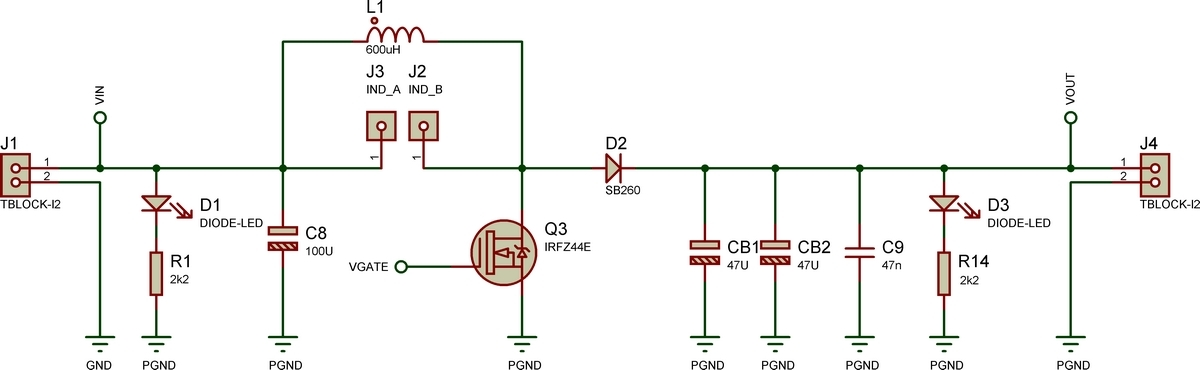
\includegraphics[width=0.95\textwidth]{sch-potencia.jpg}
	\caption{Esquemático do circuito de potência.}
	\label{fig:sch-pot}
\end{figure}

Para evitar que ruídos provenientes dos circuitos de potência (Figura \ref{fig:sch-pot}) e de chaveamento (Figura \ref{fig:sch-chaveamento}) interferissem no circuito de controle (Figura \ref{fig:sch-controle}), separou-se os terras através de componentes virtuais \emph{neckties}, como apresentado na Figura \ref{fig:neckties}. Dessa forma, cada circuito é tratado de forma individual, tendo a ligação das referências próxima ao conector de entrada (Figura \ref{fig:plano-baixa}).

\begin{figure}[H]
	\centering
	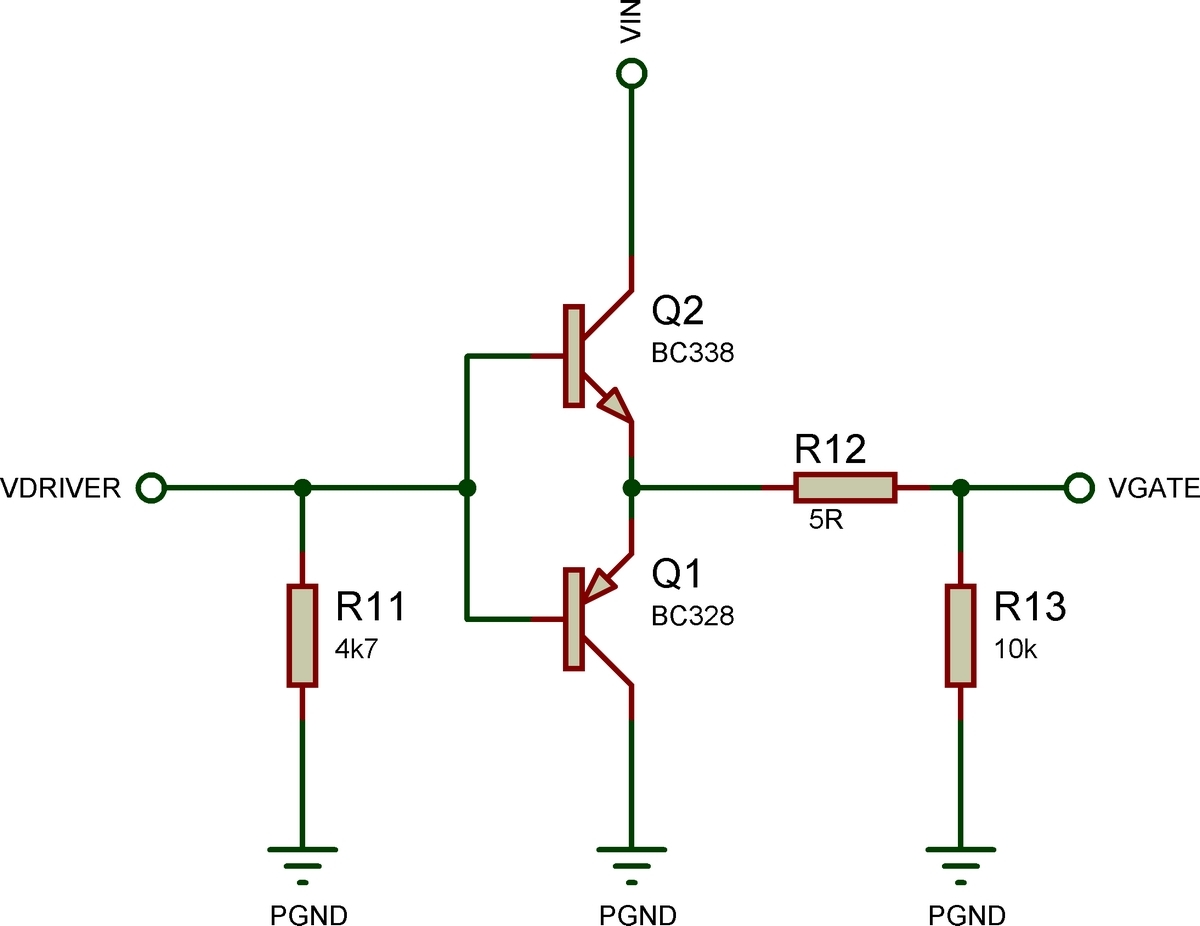
\includegraphics[width=0.5\textwidth]{sch-acionamento.jpg}
	\caption{Esquemático do circuito de chaveamento.}
	\label{fig:sch-chaveamento}
\end{figure}

\begin{figure}[H]
	\centering
	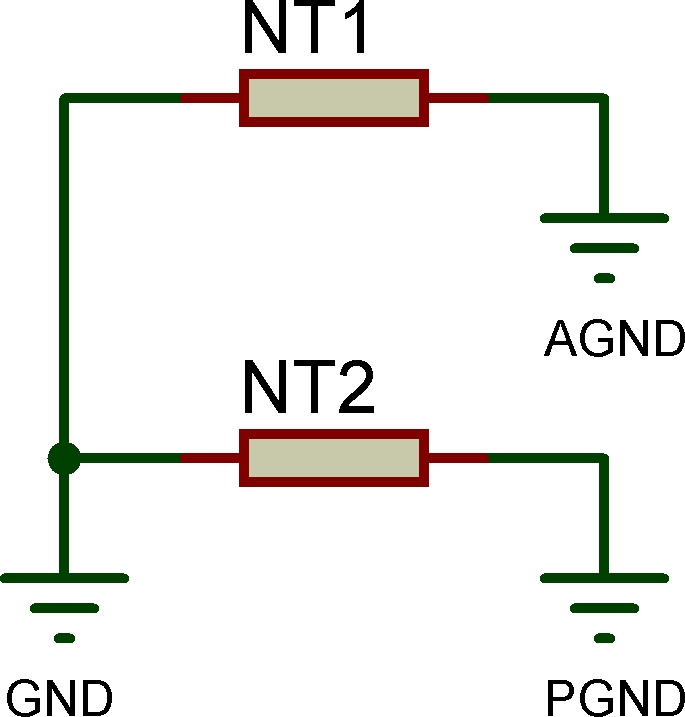
\includegraphics[width=0.28\textwidth]{sch-gnds.jpg}
	\caption{Separação dos terras de alta (PGND) e baixa (AGND) potência.}
	\label{fig:neckties}
\end{figure}

Além disso, o circuito de controle foi confinado em um pequeno plano de terra individual, como apresentado na Figura \ref{fig:plano-baixa}.

\begin{figure}[H]
	\centering
	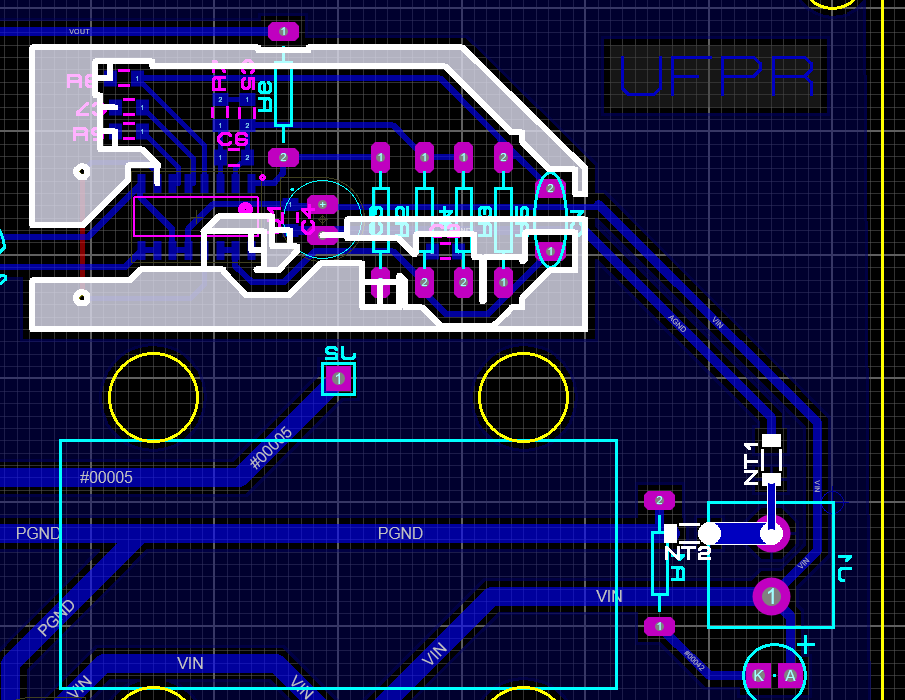
\includegraphics[width=0.82\textwidth]{pcb-ground-plane-net-tail.png}
	\caption{Destaque do plano confinado e \emph{neckties} na entrada do circuito separando os terras.}
	\label{fig:plano-baixa}
\end{figure}

Com o circuito de controle estando afastado do conector de entrada, foram colocados 2 capacitores de desacoplamento próximos ao CI TL494.

\begin{figure}[H]
	\centering
	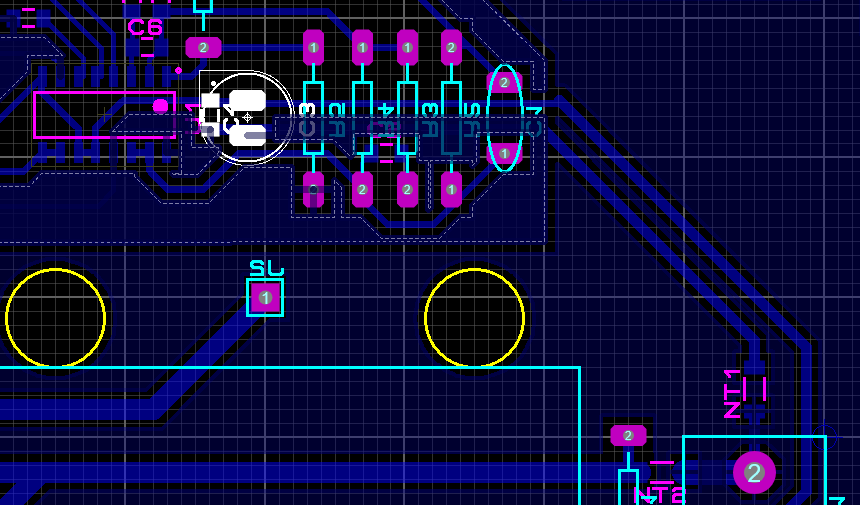
\includegraphics[width=0.82\textwidth]{pcb-caps-desacopl.png}
	\caption{Destaque dos capacitores de desacoplamento próximos ao circuito integrado.}
	\label{fig:caps-des}
\end{figure}

A Figura \ref{fig:pcb-layout} apresenta o leiaute completo e as Figuras \ref{fig:3d-top} e \ref{fig:3d-bot} apresentam as vistas superior e inferior do modelo 3D, respectivamente. Em seguida, a Figura \ref{fig:top-confec} mostra o protótipo construído.

\begin{figure}[H]
	\centering
	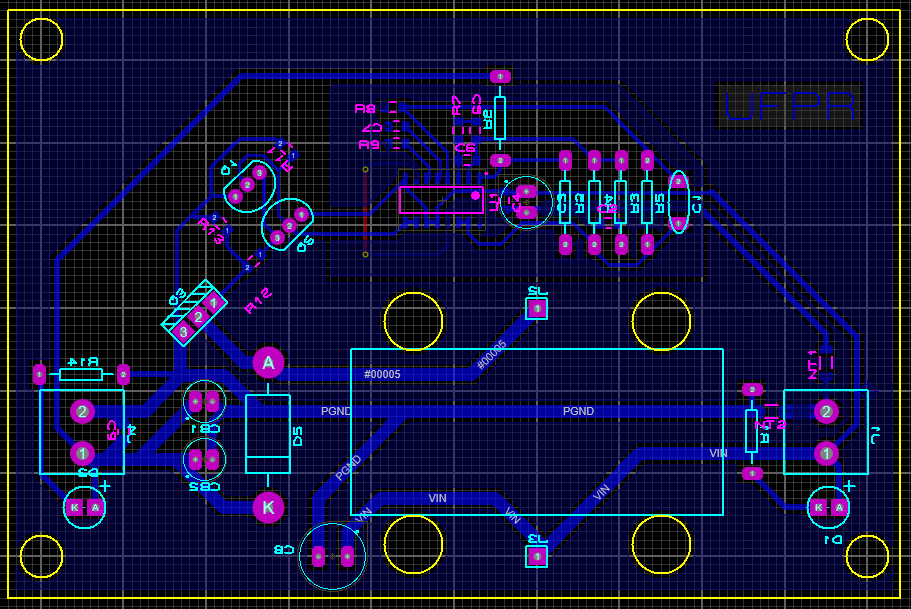
\includegraphics[width=0.87\textwidth]{pcb-layout.png}
	\caption{Leiaute da placa de circuito impresso.}
	\label{fig:pcb-layout}
\end{figure}

\begin{figure}[H]
	\centering
	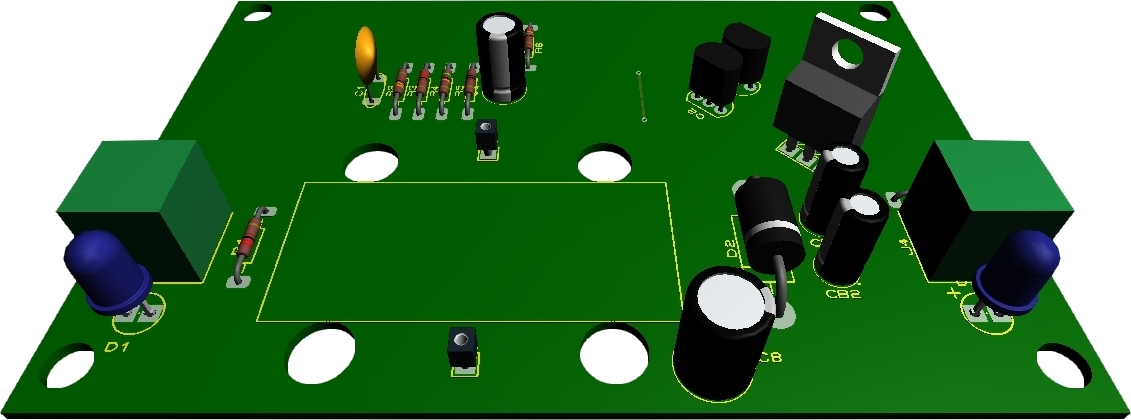
\includegraphics[width=0.87\textwidth]{3d-top.jpg}
	\caption{Vista superior do modelo 3D.}
	\label{fig:3d-top}
\end{figure}

\begin{figure}[H]
	\centering
	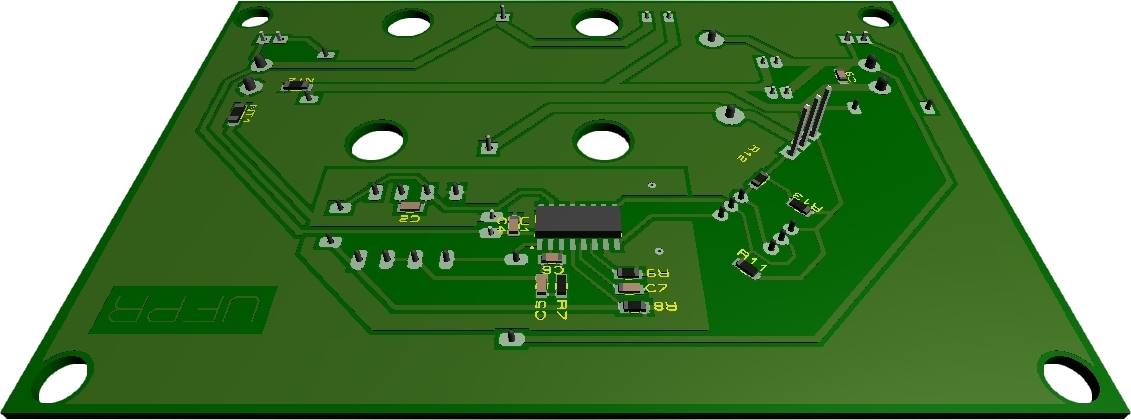
\includegraphics[width=0.9\textwidth]{3d-bottom.jpg}
	\caption{Vista inferior do modelo 3D.}
	\label{fig:3d-bot}
\end{figure}

\begin{figure}[H]
	\centering
	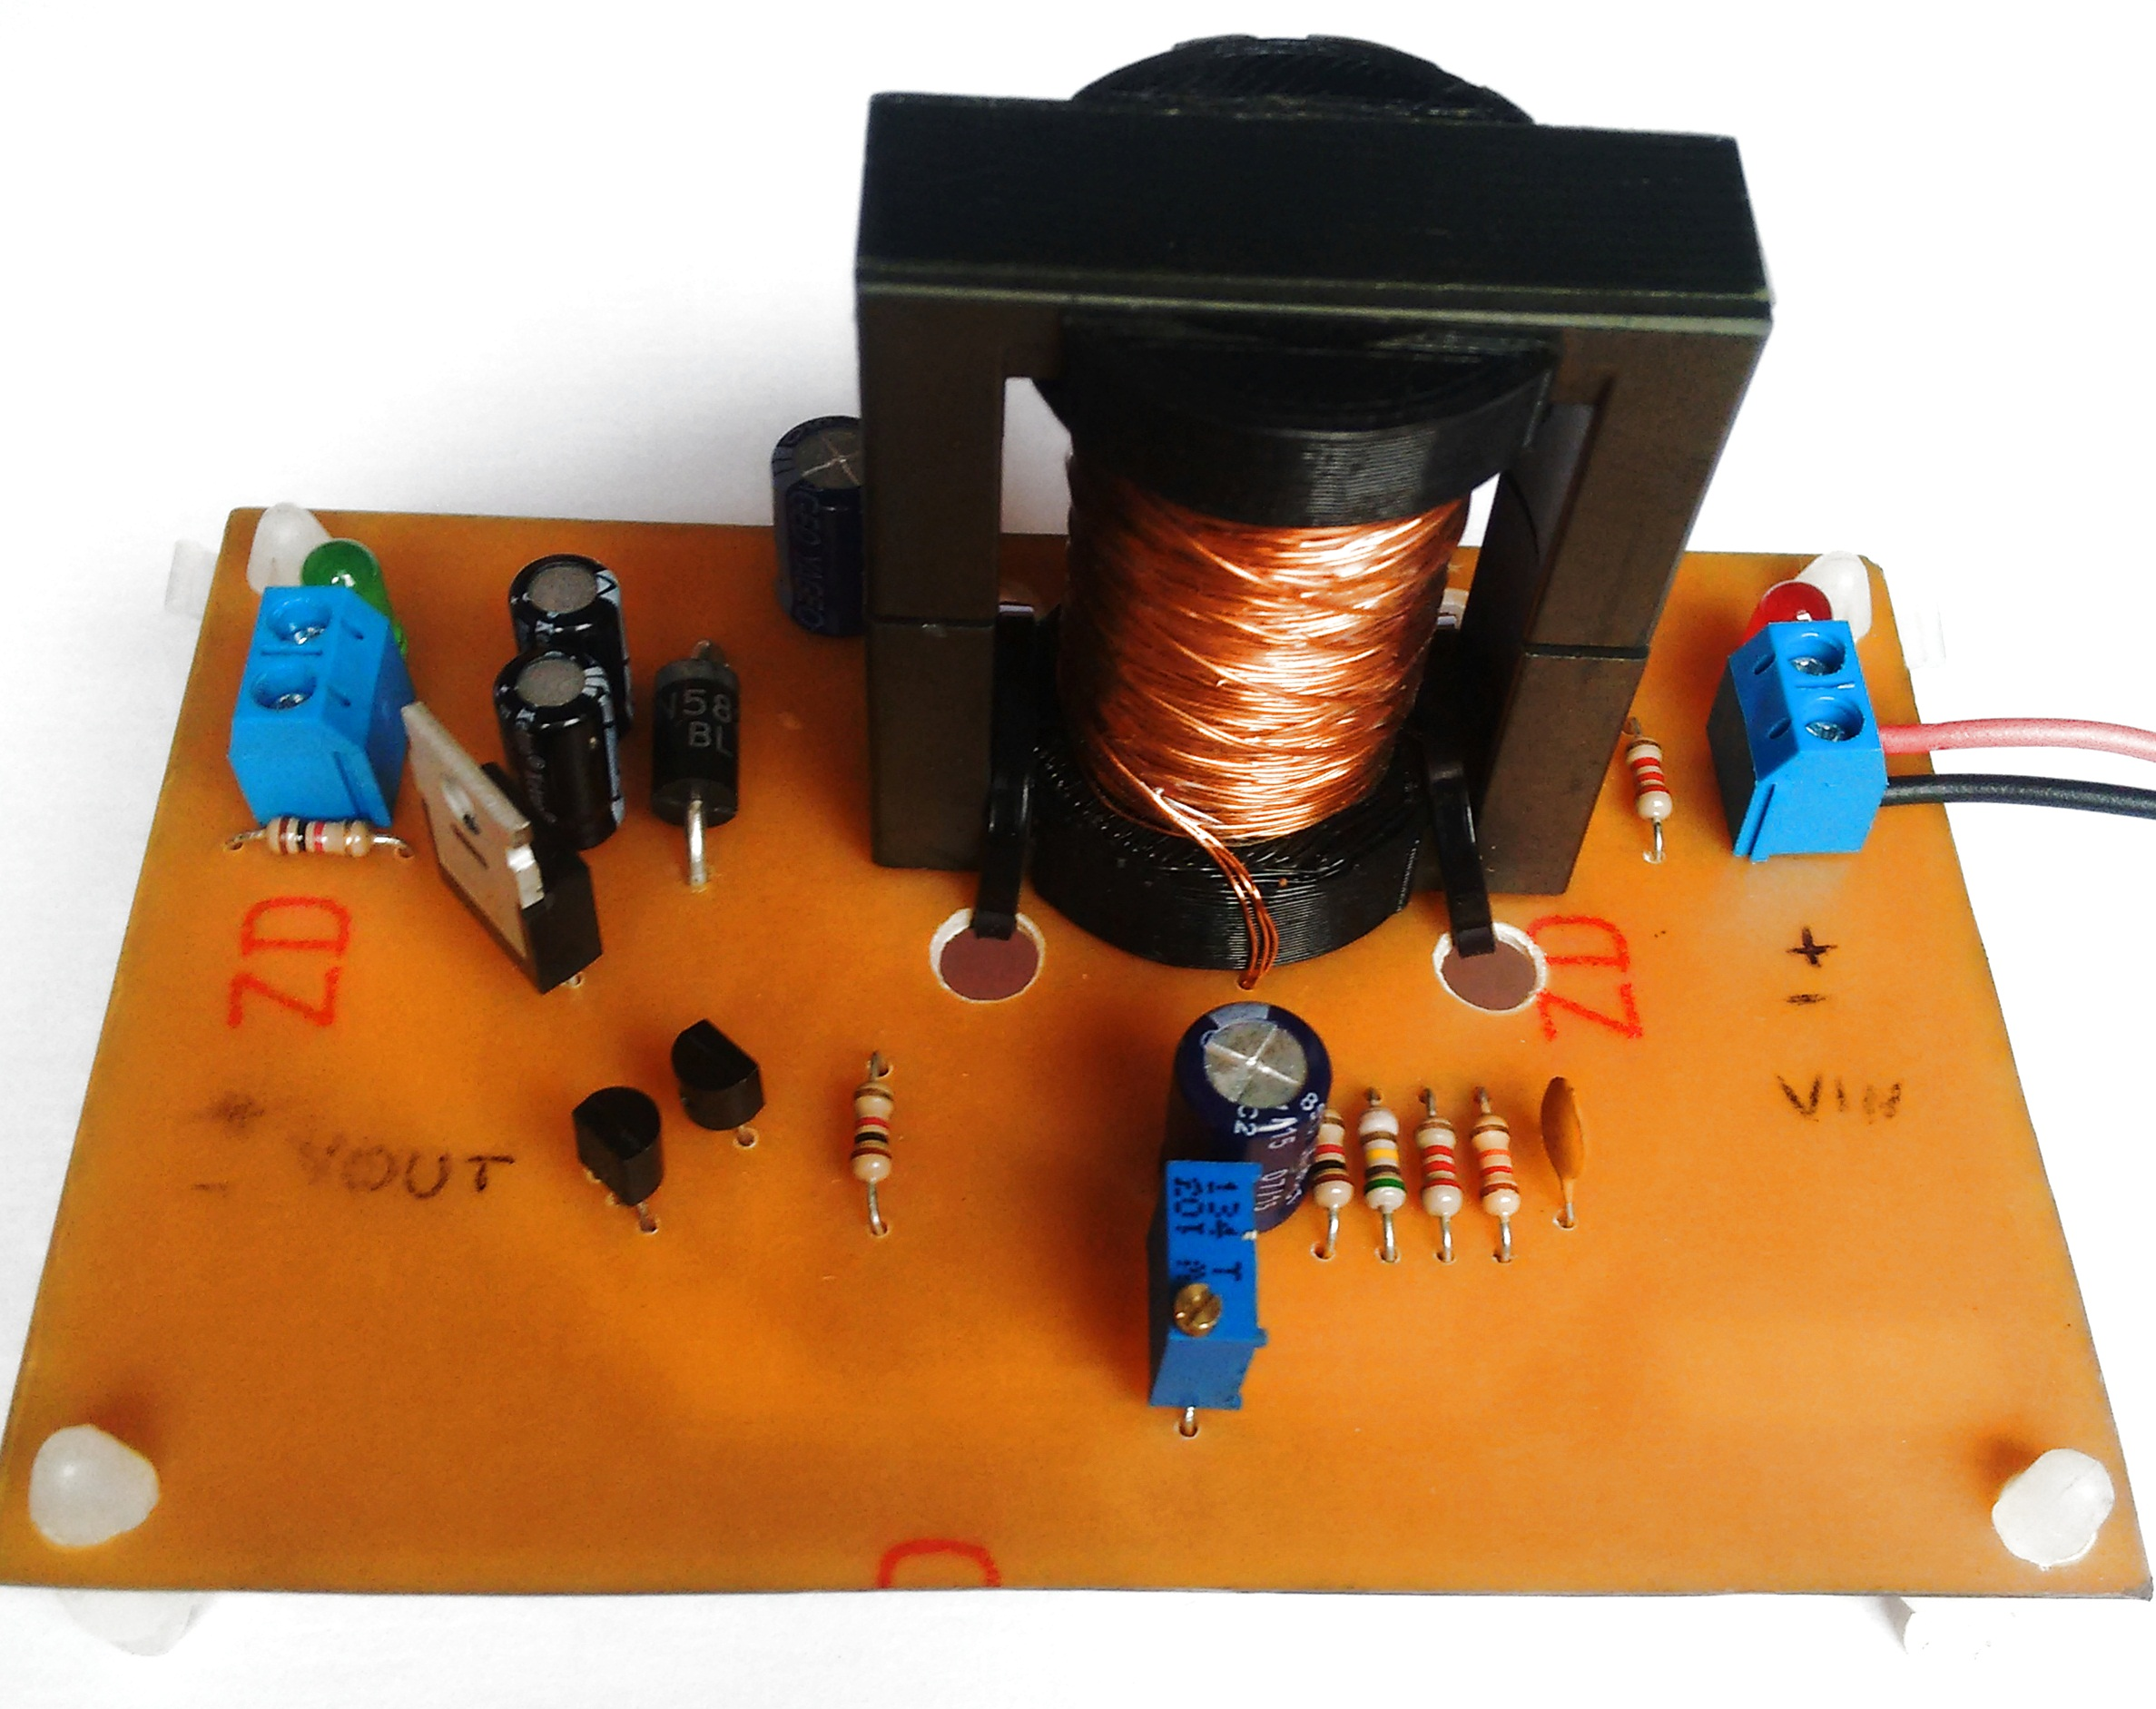
\includegraphics[width=0.75\textwidth]{c2.jpg}
	\caption{Vista superior do protótipo confeccionado.}
	\label{fig:top-confec}
\end{figure}

\clearpage

%\section{Simulação do Conversor \textit{Boost}}
%\clearpage

\section{Resultados}
\label{sec:resultados}

Os parâmetros analisados foram obtidos em 3 pontos bem definidos sobre a faixa de operação: 9V, 13,5V e 18V.

\subsection{Ondulação da tensão de saída}

As Figuras \ref{fig:ripple-18V}, \ref{fig:ripple-13v5} e \ref{fig:ripple-9V} apresentam o \emph{ripple} (ondulação) da tensão de saída para os 3 casos citados, com carga de 30W.
\FloatBarrier
\begin{figure}[H]
	\centering
	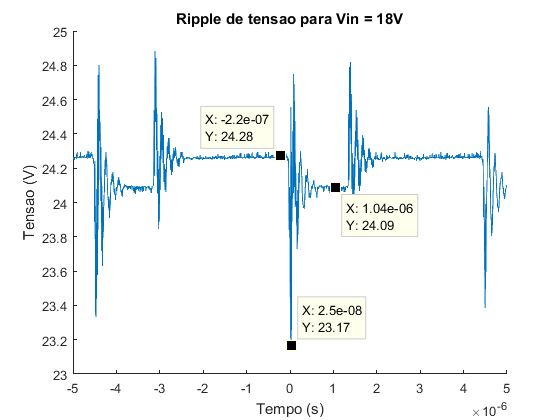
\includegraphics[width=0.8\textwidth]{ripple-vin-18V.png}
	\caption{\emph{Ripple} da tensão de saída @Vin=18V.}
	\label{fig:ripple-18V}
\end{figure}
\FloatBarrier
\begin{figure}[H]
	\centering
	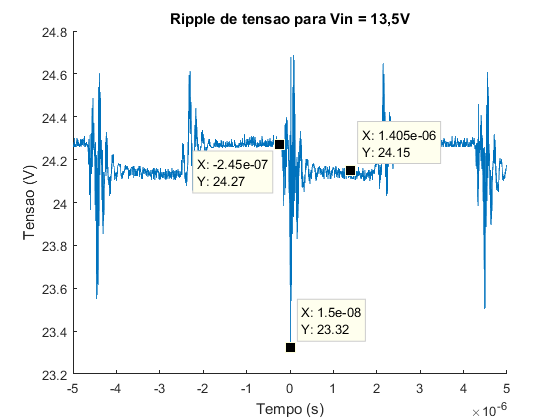
\includegraphics[width=0.8\textwidth]{ripple-vin-13V5.png}
	\caption{\emph{Ripple} da tensão de saída @Vin=13,5V.}
	\label{fig:ripple-13v5}
\end{figure}
\FloatBarrier
\begin{figure}[H]
	\centering
	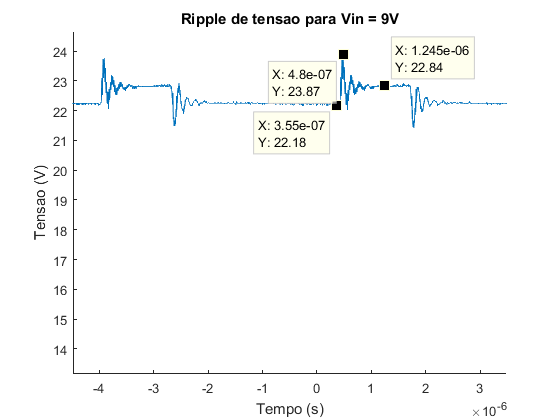
\includegraphics[width=0.8\textwidth]{ripple-vin-9V.png}
	\caption{\emph{Ripple} da tensão de saída @Vin=9V.}
	\label{fig:ripple-9V}
\end{figure}
\FloatBarrier
\subsection{Transitório para o aumento da carga}

Para esta análise, alterou-se a carga de 15W ($2 \cdot R_{Carga}~=~38,4\Omega$) para 30W ($R_{Carga} = 19,2\Omega$). As Figuras \ref{fig:trans-2R-R-18V}, \ref{fig:trans-2R-R-13V5} e \ref{fig:trans-2R-R-9V} apresentam a oscilação da tensão de saída em função da alteração brusca (degrau) da carga.

\begin{figure}[H]
	\centering
	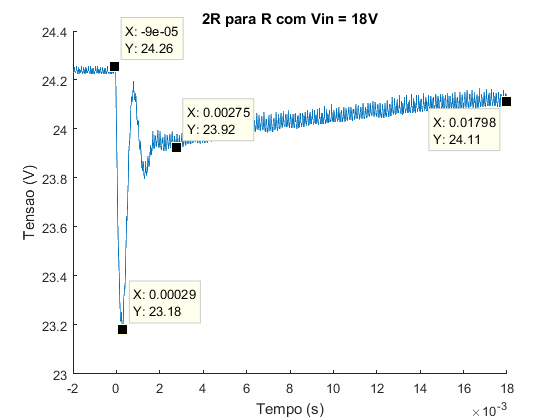
\includegraphics[width=0.8\textwidth]{2R-para-R-18V.png}
	\caption{Oscilação da tensão de saída devido a alteração brusca da carga @Vin=18V.}
	\label{fig:trans-2R-R-18V}
\end{figure}

\begin{figure}[H]
	\centering
	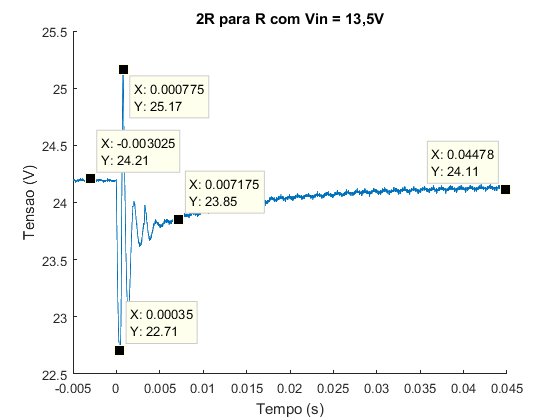
\includegraphics[width=0.8\textwidth]{2R-para-R-13V5.png}
	\caption{Oscilação da tensão de saída devido a alteração brusca da carga @Vin=13V5.}
	\label{fig:trans-2R-R-13V5}
\end{figure}

\begin{figure}[H]
	\centering
	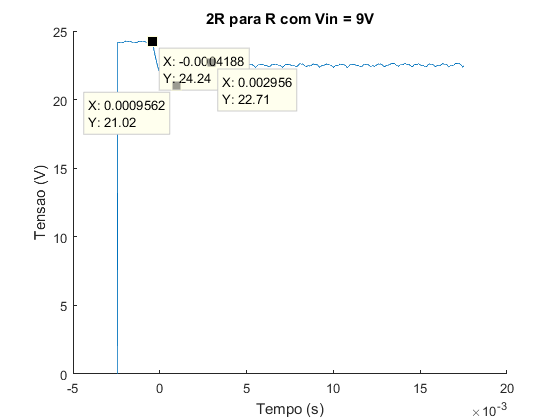
\includegraphics[width=0.8\textwidth]{2R-para-R-9V.png}
	\caption{Oscilação da tensão de saída devido a alteração brusca da carga @Vin=9V.}
	\label{fig:trans-2R-R-9V}
\end{figure}


\subsection{Transitório para a diminuição da carga}

Similar ao caso anterior, alterou-se a carga de 30W ($R_{Carga} = 19,2\Omega$) para 15W ($2 \cdot R_{Carga}~=~38,4\Omega$). As Figuras \ref{fig:trans-R-2R-18V}, \ref{fig:trans-R-2R-13V5} e \ref{fig:trans-R-2R-9V} apresentam a oscilação da tensão de saída em função da alteração brusca (degrau) da carga.

\begin{figure}[H]
	\centering
	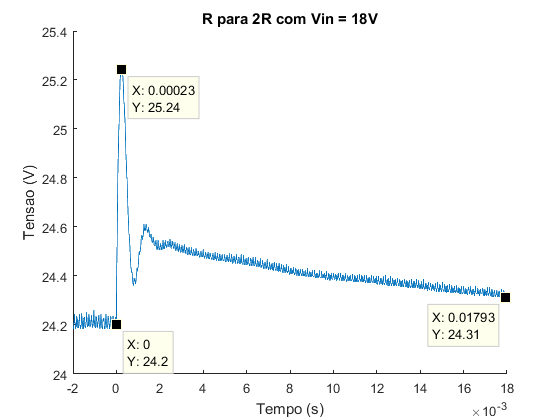
\includegraphics[width=0.8\textwidth]{R-para-2R-18V.png}
	\caption{Oscilação da tensão de saída devido a alteração brusca da carga @Vin=18V.}
	\label{fig:trans-R-2R-18V}
\end{figure}

\begin{figure}[H]
	\centering
	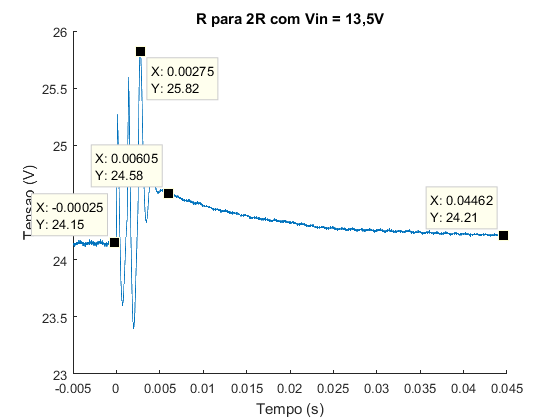
\includegraphics[width=0.8\textwidth]{R-para-2R-13V5.png}
	\caption{Oscilação da tensão de saída devido a alteração brusca da carga @Vin=13V5.}
	\label{fig:trans-R-2R-13V5}
\end{figure}

\begin{figure}[H]
	\centering
	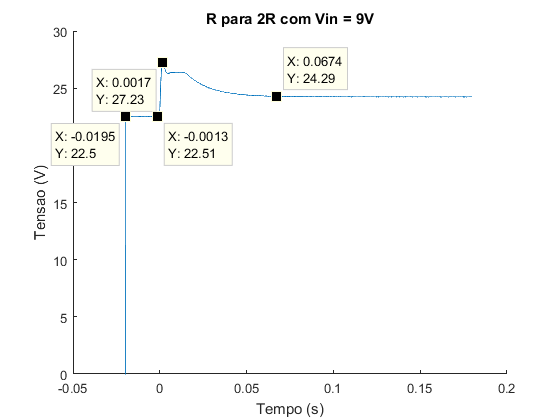
\includegraphics[width=0.8\textwidth]{R-para-2R-9V.png}
	\caption{Oscilação da tensão de saída devido a alteração brusca da carga @Vin=9V.}
	\label{fig:trans-R-2R-9V}
\end{figure}

\subsection{Tensão dreno-fonte}
\label{subsub:vds}

As Figuras \ref{fig:vds-18V}, \ref{fig:vds-13V5} e \ref{fig:vds-9V} apresentam a tensão dreno-fonte do Mosfet, também para os 3 casos citados.

\begin{figure}[H]
	\centering
	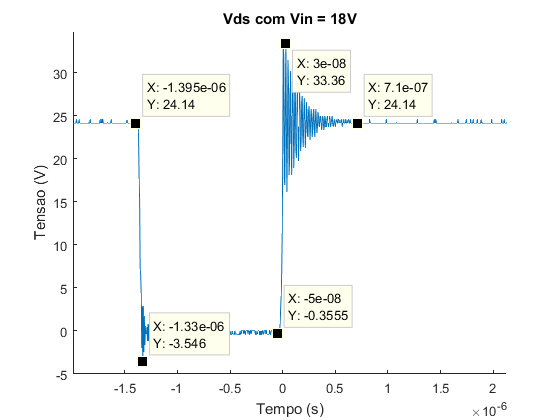
\includegraphics[width=0.8\textwidth]{vds-18V.png}
	\caption{Tensão dreno-fonte para @Vin=18V.}
	\label{fig:vds-18V}
\end{figure}

\begin{figure}[H]
	\centering
	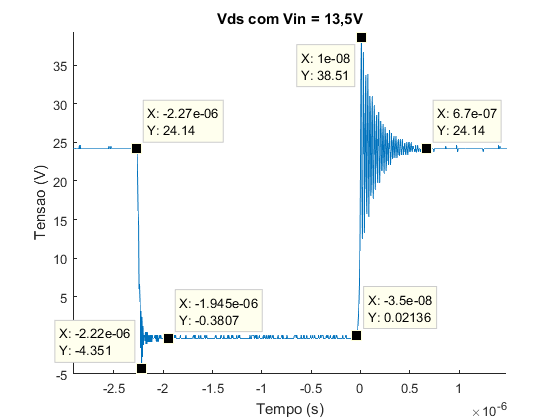
\includegraphics[width=0.8\textwidth]{vds-13V5.png}
	\caption{Tensão dreno-fonte para @Vin=13V5.}
	\label{fig:vds-13V5}
\end{figure}

\begin{figure}[H]
	\centering
	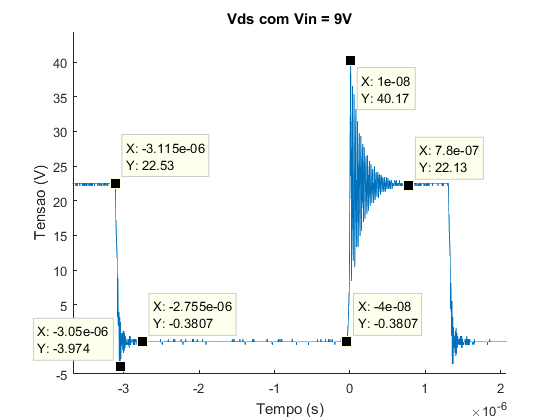
\includegraphics[width=0.8\textwidth]{vds-9V.png}
	\caption{Tensão dreno-fonte para @Vin=9V.}
	\label{fig:vds-9V}
\end{figure}


\clearpage

\section{Conclusões}
\label{sec:conclusoes}

Como se pôde notar na Seção \ref{sec:resultados}, o conversor \emph{Boost} não atendeu todas as especificações de projeto. Um indicativo de que havia algo errado foi o fato do indutor estar aquecendo consideravelmente. Ao percebê-lo, reviram-se os cálculos e notou-se que as correntes eficaz e de pico levadas em conta nas Equações \ref{eq:b-max-erro} e \ref{eq:area-erro} estão mal levantadas. O correto seria ter considerado os valores de pico da simulação (Seções \ref{subsub:corrente-media} e \ref{subsub:corrente-max}). Com o indutor aquecendo, o material do carretel, produzido em impressora 3D, começou a amolecer. Isso causou a diminuição do entreferro (devido ao peso do núcleo estar sobre o carretel), levando à saturação. Com o núcleo saturado, o indutor não conseguia fornecer a corrente necessária para suprir a demanda. Com isso, percebe-se que, nos casos em que há maior demanda de corrente (por exemplo, Figura \ref{fig:ripple-9V}), a tensão de saída fica muito abaixo dos 24V esperados.

Observou-se também que a simulação apresentou valores não condizentes com o caso real. Como pode-se notar na Seção \ref{subsub:vds}, os valores das tensões entre dreno e fonte foram maiores que os apresentados na
Seção \ref{subitem:vds}. Por sorte, os valores reais estavam dentro do limite suportado pelo \emph{Mosfet}.

\end{document}
